\documentclass[tikz]{standalone}
\usepackage{units}
\usepackage{calc}
\begin{document}

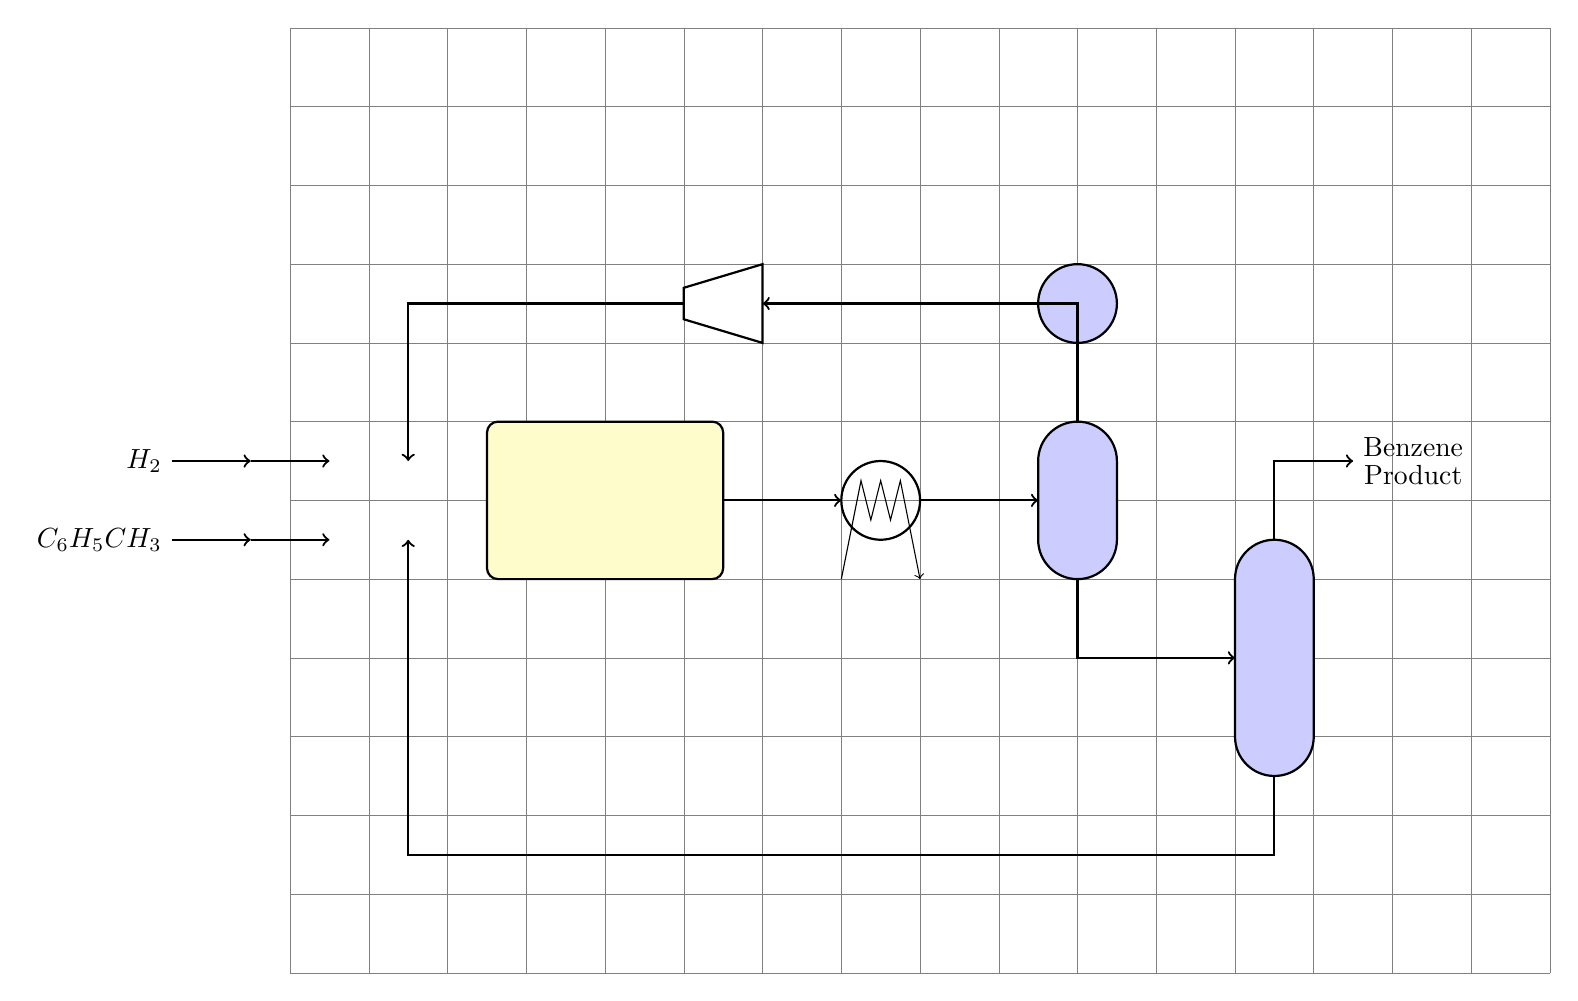
\begin{tikzpicture}
  \draw[step=1cm,gray,very thin] (0,0) grid (16,12);
  
  % Coordinates
  \coordinate (reactor) at (2.5,6);
  \coordinate (Hfeed) at (-1.5,6.5);
  \coordinate (Tfeed) at (-1.5,5.5);
  \coordinate (hx) at (7,6);
  \coordinate (flash) at (9.5,6);
  \coordinate (dist) at (12,4);
  \coordinate (compressor) at (6,8.5);
  \coordinate (purge) at (10,8.5);
  
  % Reactor
  \draw[thick,fill=yellow!20,rounded corners] (reactor) -- ++(0,1) 
    -- ++(3,0) -- ++(0,-2) -- ++(-3,0) -- cycle;
    
  % Heat Exchanger. Given location of the feed port, draws an exchanger
  % with outlet at ++(1,0) and coolant ports at ++(0,-1) and ++(1,-1).
  \draw[thick] (hx) arc(+180:-180:0.5cm);
  \draw [->] (hx) ++(0,-1) -- ++ (0.25,1.25) -- ++(0.125,-0.5) -- ++(0.125,0.5)
    -- ++(0.125,-0.5) -- ++(0.125,0.5) -- ++(0.25,-1.25);
    
  % Flash
  \draw[thick,fill=blue!20] (flash) -- ++(0,.5) arc(180:0:0.5cm) -- ++(0,-1)
    arc(0:-180:0.5cm) -- ++(0,.5);

  % Distillation
  \draw[thick,fill=blue!20] (dist) -- ++(0,1) arc(180:0:0.5cm) -- ++(0,-2)
    arc(0:-180:0.5cm) -- ++(0,1);

  % Compressor
  \draw[thick] (compressor) -- ++(0,0.5) -- ++(-1,-0.3) -- ++(0,-0.4) --
    ++(1,-0.3) -- ++(0,0.5);
    
  % Purge
  \draw[thick,fill=blue!20] (purge) circle (0.5cm);
    
  % Lines
  \draw[->,thick] (Hfeed) node [left] {$H_2$} -- ++(1,0);
  \draw[->,thick] (Hfeed) ++(1,0) -- ++(1,0);
  \draw[->,thick] (Tfeed) node [left] {$C_6H_5CH_3$} -- ++(1,0);
  \draw[->,thick] (Tfeed) ++(1,0) -- ++(1,0);
  
  \draw[->,thick] (compressor) ++(-1,0) -- ++(-3.5,0) -- ++(0,-2);
  \draw[->,thick] (reactor) ++(3,0) -- (hx);
  \draw[->,thick] (hx) ++(1,0) -- (flash);
  \draw[->,thick] (flash) ++(0.5,1) -- ++(0,1.5) -- (compressor);
  \draw[->,thick] (flash) ++(0.5,-1) -- ++(0,-1) -- (dist);
  \draw[->,thick] (dist) ++(0.5,-1.5) -- ++(0,-1) 
    -- ++(-11,0) -- ++(0,4);
  \draw[->,thick] (dist) ++(0.5,1.5) -- ++(0,1) -- ++(1,0)
    node[right] {\shortstack{Benzene\\ Product}};

 
\end{tikzpicture}

\end{document}